\documentclass[12pt,letterpaper]{article}
\usepackage{graphicx}
\usepackage{multirow}
\usepackage{authblk}
\usepackage{float}
\usepackage{rotating}
\usepackage{url}
\usepackage{lscape}
\usepackage{longtable}
\usepackage{subfig}
\usepackage{natbib}
\usepackage{lineno}
\usepackage{amsmath,amsthm}
%\usepackage{fullpage}
\usepackage{anysize}
\marginsize{1.0in}{1.0in}{1.0in}{1.0in}
\linespread{1.6}

\newcommand{\Pic}[2][0.85]{\begin{center}\includegraphics[width=0.8\textwidth,height=#1\textheight,keepaspectratio]{#2}
 \end{center} }


\title{Digital Elevation Models (DEMs) clustering for terrain modeling}
\author[1]{ E. R. Stefanescu }
\author[1]{A.K. Patra}
\author[2]{M. Bursik}
\affil[1]{Department of Mechanical and Aerospace Engineering, University at Buffalo, Buffalo, NY 14260}
\affil[2]{Department of Geology, University at Buffalo, Buffalo, NY 14260 }

\date{\today}


\begin{document}
\linenumbers
\maketitle

\begin{abstract}
We consider the problem of Digital Elevation Models (DEMs) segmentation 
in homogeneous regions, aiming for identification of plateaux, ridges, small drainages,
straight front slopes, valleys, and crests.  
In the paper we explore and compare different methods 
for the segmentation that are required / needed when we want to construct a 
sparse representation of the DEM.  Methods that are extensively and successfully used in image segmentation such as Spatial Gaussian Mixture Model and Spectral Clustering are adapted for the case in which each data point has associated range of geomorphometric measures. These are two complex methods which account for the spatial correlation of the elevation points and have the advantage that they can be used for almost any application where relationships between topographic features and 
other components of landscapes are to be assessed.
\end{abstract}

\section{Introduction}
Information about topography is necessary for landscape evaluation, erosion studies,
hydrology and geophysical modeling, natural hazard prevention, etc. The classic way to 
incorporate relief units into a landscape assessment is to delineate them during field survey
or using stereo aerial photographs. This approach is relatively time-consuming and the results
depend on the subjective decision of the interpreter.
Several methods for the creation of landform elements using elevation-derived attributes are
described in the literature. Commonly, these techniques developed regions of homogeneity based
on common attributes and then classified those regions (or groups of regions) as elements. The most widely used techniques
are: watershed segmentation, object-based image analysis, support vector machine, segmentation
using heuristic rules and fuzzy logic, fuzzy $K$-means classification and self organizing map. Many of these
techniques have drawbacks, especially when the method relies heavily on hydrological information and 
requires data-specific knowledge; also these methods don't incorporate autocorrelation between 
the same attribute at two locations in their models.
Digital Elevation Models (DEMs) are digital representations of terrain, and are represented as an array of 
squared cells (data points/ pixels) with an elevation associated to each data point. They can have
different resolutions (5m, 30m, 90m, 120m, etc) and can be obtained from various methods 
(photometry, radar interferometry, laser altimetry, etc.). Usually the size of a DEM varies from
tens to hundreds of kilometers which can lead to thousands to millions of grid points. 
 
In this context, we would like to implement a more complex model segmentation of a DEM of Mammoth Mountain to create non-overlapping groupings of homogeneous regions. Mammoth Mountain (Fig.~\ref{fig:fig1}) is a volcano located in California and it was chosen due to the ease of obtaining data sets. 
\begin{figure}[ht!]
\center
      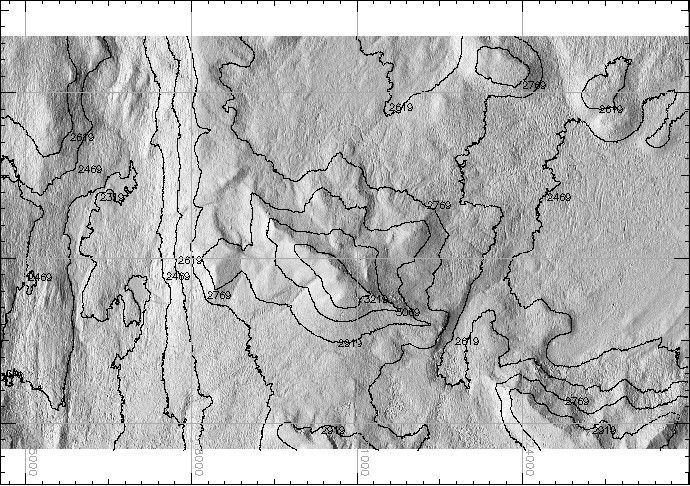
\includegraphics[width=10cm,height=11cm,keepaspectratio]{figs/Topsar5.png}\\
  \caption{Hillshade plot of the Mammoth Mountain  }\label{fig:fig1}
\end{figure}

\section{Methodology}
Segmentation methods are based on some data point or region similarity
in relation to their local neighborhood. A variety of different methods have been proposed
for image segmentation such as boundary-based segmentation, region-based segmentation
and pixel-labeling. Recently, Expectation-Maximization (EM) algorithm has attracted considerable
interest to compute the maximum likelihood estimates, when the observations are unlabeled. 
The unsupervised clustering techniques do not require training data, but they do require an initial
segmentation.

\subsection{Spatial Gaussian Mixture and the Expectation-Maximization algorithm}
To be able to perform the segmentation of the DEM in homogeneous regions
we need to specify a range of geomorphometric measures which can be extracted
from the surface. We define a \textit{feature matrix} of DEM attributes, consisting of elevation and 
first and second derivatives of elevation (slope, profile curvature and tangential curvature).
Slope and curvature are easily extracted from a DEM within a Geographical Information System (GIS).

The major drawback of traditional mixture models is lack of spatial correlation in the clustering processing.
Sujaritha et. al. proposed an adaptive Spatial Gaussian Mixture Model and EM algorithm which introduces the spatial information into the clustering process. The technique, described below, is what we attempted to implement for our case in which we are dealing with a feature matrix and not a vector in color space. \\

%We implement an Expectation Maximization (EM) algorithm through Gaussian Mixtures (GM). In order to implement the GM approach, we first needed to determine the [believed] number of components present within our data and assume that each of these components contains data of the Gaussian form.
%Our data is represented as a matrix with implied spatial relations and as such our EMGM approach considers membership likelihood based upon probability as well as location. However, this does not imply that two spatially separate points are unable belong to the same class, but rather that it is more unlikely that they will. In our approach, we systematically apply the Expectation and Maximization steps to each data point until convergence by utilizing the a priori probability and maximizing membership likelihood.

\textit{Gaussian Mixture Model}

To define a Gaussian mixture model with $K > 1$ components in $\mathcal{R}^D$ for $D\ge1$, let $x_n$ be the observation of the $n$th data point of a DEM. The density function $p(x_n)$ is given by:
\begin{align}
 p(x_n) = \sum_{k=1}^{K}\pi_k\mathcal{N}(x_n | \mu_k, \Sigma_k)
\end{align}
where $\pi_1, \pi_2 \cdots \pi_k$ are the mixing coefficients and $\mu_k$, $\Sigma_k$ are the Gaussian distribution's parameters
for each $k$th component.
The mixing coefficients satisfy the following conditions:
\begin{align}
0\le\pi_k\le1 \;  \; , \; \;\sum_{k=1}^{K}=1
\end{align}
For the Gaussian mixtures, each component density is a Gaussian probability with $\mu_k$ and
covariance $\Sigma_k$:
\begin{align}
p(x_n) = \mathcal{N}(x_n | \mu_k, \Sigma_k) = \frac{1}{2\pi^{\frac{D}{2}}}\frac{1}{\det(\Sigma_k)^{\frac{1}{2}}} \exp\lbrace-\frac{(x_n - \mu_k)^T(x_n - \mu_k)}{2\Sigma_k}\rbrace
\end{align}

The inherent steps of the EM for the Gaussian mixture approach can be summarized as:
\begin{itemize}
\item Initialize the means $\mu_k$, covariance $\Sigma_k$, mixing coefficients $\pi_k$ and the log likelihood.
\item \textbf{E step} evaluate the responsibilities using the current parameters values:
\begin{align}
\gamma(z_{nk} )= \frac{\pi_k \mathcal{N}(x_n | \mu_k, \Sigma_k)}{\sum_{j=1}^{K}\pi_j\mathcal{N}(x_n |\mu_j, \Sigma_j)}
\end{align}
\item \textbf{M step} Re-estimate the parameters using the current responsibilities:
\begin{align}
&\mu_k^{new} = \frac{1}{N_k}\sum_{i=1}^N \gamma(z_{nk})x_n \\
&\Sigma_k^{new} =  \frac{1}{N_k}\sum_{i=1}^N \gamma(z_{nk})(x_n - \mu_k^{new})(x_n - \mu_k^new)^T \\
&\pi_k = \frac{1}{N}\sum_{n=1}^{N}\gamma(z_{nk} )
\end{align}
\item Evaluate the log likelihood:
\begin{align}
\ln p(X | \mu,\Sigma,\pi) = \sum_{n=1}^{N}\ln \lbrace\sum_{k=1}^{K}\pi_k \mathcal{N}(x_n|\mu_k, \Sigma_k)\rbrace
\end{align}
\end{itemize}

\textit{Adaptive Spatial Gaussian Mixture Model}

In the paper by Sujaritha et.al., a way of incorporating spatial relationships was proposed. Therefore, in the calculation 
of the density function, the data point $x_n$ will be influenced by its neighbors.
 
 \begin{align}
p(x_n) = \frac{1}{2\pi^{\frac{D}{2}}}\frac{1}{\det(\Sigma_k)^{\frac{1}{2}}} \nonumber
&\times [\exp\lbrace-[\frac{\eta_n^k(x_n - \mu_k)^T(x_n - \mu_k)}{2\Sigma_k} \\
&+ \frac{\eta_n^k}{8} \sum_{X_l \in X_{x_n}} 
 \frac{(x_n - \mu_k)^T(x_n - \mu_k)}{2\Sigma_k} ]\rbrace]
\end{align}

where $\eta_n$ is the parameter that controls the neighbors influence and $X_{x_n}$ is the subset of 
neighborhood data points of $x_n$ in a $3\times3$ window. $\eta_n$ is calculated using the following formula:
\begin{align}
\eta_i^k = df_{std}^{k}(i)/x_{std}(i)
\end{align}
where
\begin{align}
df_{std}^{k}(i) = (\frac{1}{9} [ \sum_{X_l \in X_{x_n}} \lbrace ( df_{x_n}^k - \mu)^2\rbrace + (df_{x_i}^k - \mu)^2])^{1/2}
\end{align}
$\mu$ is the mean value of $df$ in the $3\times3$ window:
\begin{align}
df_{x_n}^{k} = (\frac{(x_n - \mu_k)^T(x_n - \mu_k)}{2\Sigma_k} 
\end{align}
In order to eliminate the unbalanced effect on the weighting functions between smooth and sharp edges,
the $df$ is divided by the standard deviation of all the data points in the $3\times3$ window
\begin{align}
x_{std}(i) = \lbrace (\frac{1}{9} \sum_{X_l \in X_{x_n}} (x_l - \hat{x})^2 + (x_n - \hat{x})^2)\rbrace ^{1/2}
\end{align}
\subsection{$K$-means}
Since $EM$ algorithm convergences to local maxima, initialization is very important. The initialization 
of the Gaussian mixture parameters is done using $K$-means.
$K$-means is essentially a sorting and binning procedure where the user determines the number 
of bins / clusters to be used and the rules for sorting. The
$K$-means procedure sorts a set of data points into a specified number of clusters based on the 
feature vector for each data point [3].
Comparison of the $K$-means algorithm with the $EM$ algorithm for Gaussian mixtures shows that they are
very similar [6]. The $K$-means algorithm uniquely assigns each data point within a cluster whereas the$EM$ algorithm makes
the assignment based on the posterior probabilities.
The data set available is a 5m DEM, covering an area of $\approx 94 km^2$ which results in $\approx 3$ millions 
data points. To speed up the computational time, the majority of the analysis was performed on a decimated 
DEM having a 120m resolution and 6550 data points. 
The following steps are implemented for the $K$-means algorithm:
\begin{itemize}
\item We choose $k$ = 4, 6 and 10 clusters from the DEM. There are $\mu_1, \mu_2, \cdots , \mu_k$ means 
that we use for initialization.
\item For each elevation point the nearest mean is calculated.
\begin{align}
c_{i} = \underset{\mu_j \in \{\mu_1, \mu_1, \cdots, \mu_k \}}{\operatorname{argmax}} (x_i - \mu_j)^2
\end{align}
\item The means values were updated based on the elevation points assigned to them. 
\item The above steps were repeated until the locations of the means were no longer changing
by a significant amount.
\end{itemize}
%The K-means was performed on the \textit{feature matrix} $X = \{x_k | 1\le k \le N\}$ with dimensionality $d$,
%where $x_k$ is a $d \times 1$ matrix. In this case $d=4$ and $N=6550$. We have chosen random centroids 
%from the DEM and the resulting clusters for different $k$ are presented in Figure~\ref{fig:fig2} (a,b,d). Based on 
%the hillshade plot of the DEM (Fig.~\ref{fig:fig1}), we were able to pick 6 centroids and performed another K-means
%analysis. The results seen in Fig.~\ref{fig:fig2} (c) and Fig.~\ref{fig:fig2} (b) are very similar and we can conclude that
%for this DEM, with this particular geomorphometric measures, the k-means converges and it is independent on the 
%initialization means. 

\subsection{Spectral Clustering}
A digital representation of a terrain surface is an approximation of
reality and is often subject to significant error. The error is
usually not known in terms of both magnitude and spatial distribution.
There are, in fact large uncertainties associated with the construction
of DEMs. DEM vendors generally provide users with a
measure of vertical accuracy in the form of the root mean squared
error (RMSE) statistic.
One key feature of the DEM grid points, which are spatial data, is the 
autocorrelation of observations in space.  Generally, spatial autocorrelation refers to the
correlation between the same attribute at two locations. Observations
in close spatial proximity tend to be more related than observations at larger distances or separation. Based on this
assumption our next clustering method will be Spectral Clustering [2]-[4]. %\citep{Ng_Jordan, Luxburg}.

Spectral Clustering has been used with success in the field of computer vision for data clustering. Compared with
traditional clustering algorithms, Spectral Clustering has some advantages: it can recognize the clusters of unusual
shapes and obtain the globally optimal solutions in a continuous domain by eigendecomposition [5]. This property makes
Spectral Clustering more suitable for many applications, such as speech separation, image segmentation, large scale integration design, and so on.

The main idea of Spectral Clustering is to build a weighted graph $G(V,E)$, where $V$ represents vertices and $E$, edges. 
We represent each elevation point as a node in the graph $G$ and the links between the adjacent data points will form the edges of the graph. Like other clustering algorithms, Spectral Clustering attempts to partition data points into groups such that the 
members of a group are similar to each other and dissimilar to data points outside of the group. Spectral clustering has
a simple formulation and can be solved by standard linear algebra techniques, however, it typically produces better
results than traditional clustering methods such as $K$-means and mixture models [6]-[7]
Given data points, an affinity matrix can be represented by a weighted adjacency matrix $W$, where $w_{ij}$ is a measure
of the similarity between $x_i$ and $x_j$. The affinity matrix is used to preserve the local structure of the patterns. It expresses the degree of similarity between points, and
it must have the following properties: i) non-negative; ii) symmetric; iii) invertible.
We have chosen the heat kernel for calculating the affinity matrix, as:
%\begin{align}
%W_{i,j} = \exp ( -  \frac{\lVert x_i - x_j \rVert^2}{\sigma^2} )
\begin{equation}
{\mathbf W_{ij}} = \left\{
\begin{array}{rl}
\exp{\frac{- \parallel F(i) - F(j) \parallel}{\sigma_F^2}}*exp{\frac{- \parallel x(i) - x(j) \parallel}{\sigma_x^2}}, & if \parallel x(i) - x(j) \parallel \le r\\
0, & \qquad \text{otherwise},
\end{array} 
\right.
\end{equation} where $F(i)$ represents the DEM feature vector for node $i$, and $x(i)$ represents the coordinate location of $i^{th}$ node.
%\end{align}
where $\sigma > 0$ is a tuning parameter that controls the decay of the affinity [8].
The degree $d_i$ of node $i$ is the sum of all edge weights incident on $x_i$:
\begin{align}
d_i = \sum_{j=1}^n w_{ij}
\end{align} 
The graph Laplacian matrix is defined as:
\begin{align}
L = D - W
\end{align}
$L$ satisfies the following properties:
\begin{itemize}
\item For every $f \in \mathcal{R}^n$ we have :
\begin{equation}
f' L f = \frac{1}{2} \sum_{i,j=1}^n w_{ij}(f_i - f_j)^2.
\end{equation}
\item $L$ is symmetric and positive semi-definite.
\item The smallest eigenvalue of $L$ is $0$ and the corresponding eigenvector is the constant unity vector $1$.
\item $L$ has $n$ non-negative, real-valued eigenvalues $0=\lambda_1 \le \lambda_2 \le \cdots \le \lambda_n$.
\end{itemize}
The steps involved in segmentation using Spectral Clustering are summarized in Figure ~\ref{fig:fig2}.
\begin{figure}[ht!]
\center
      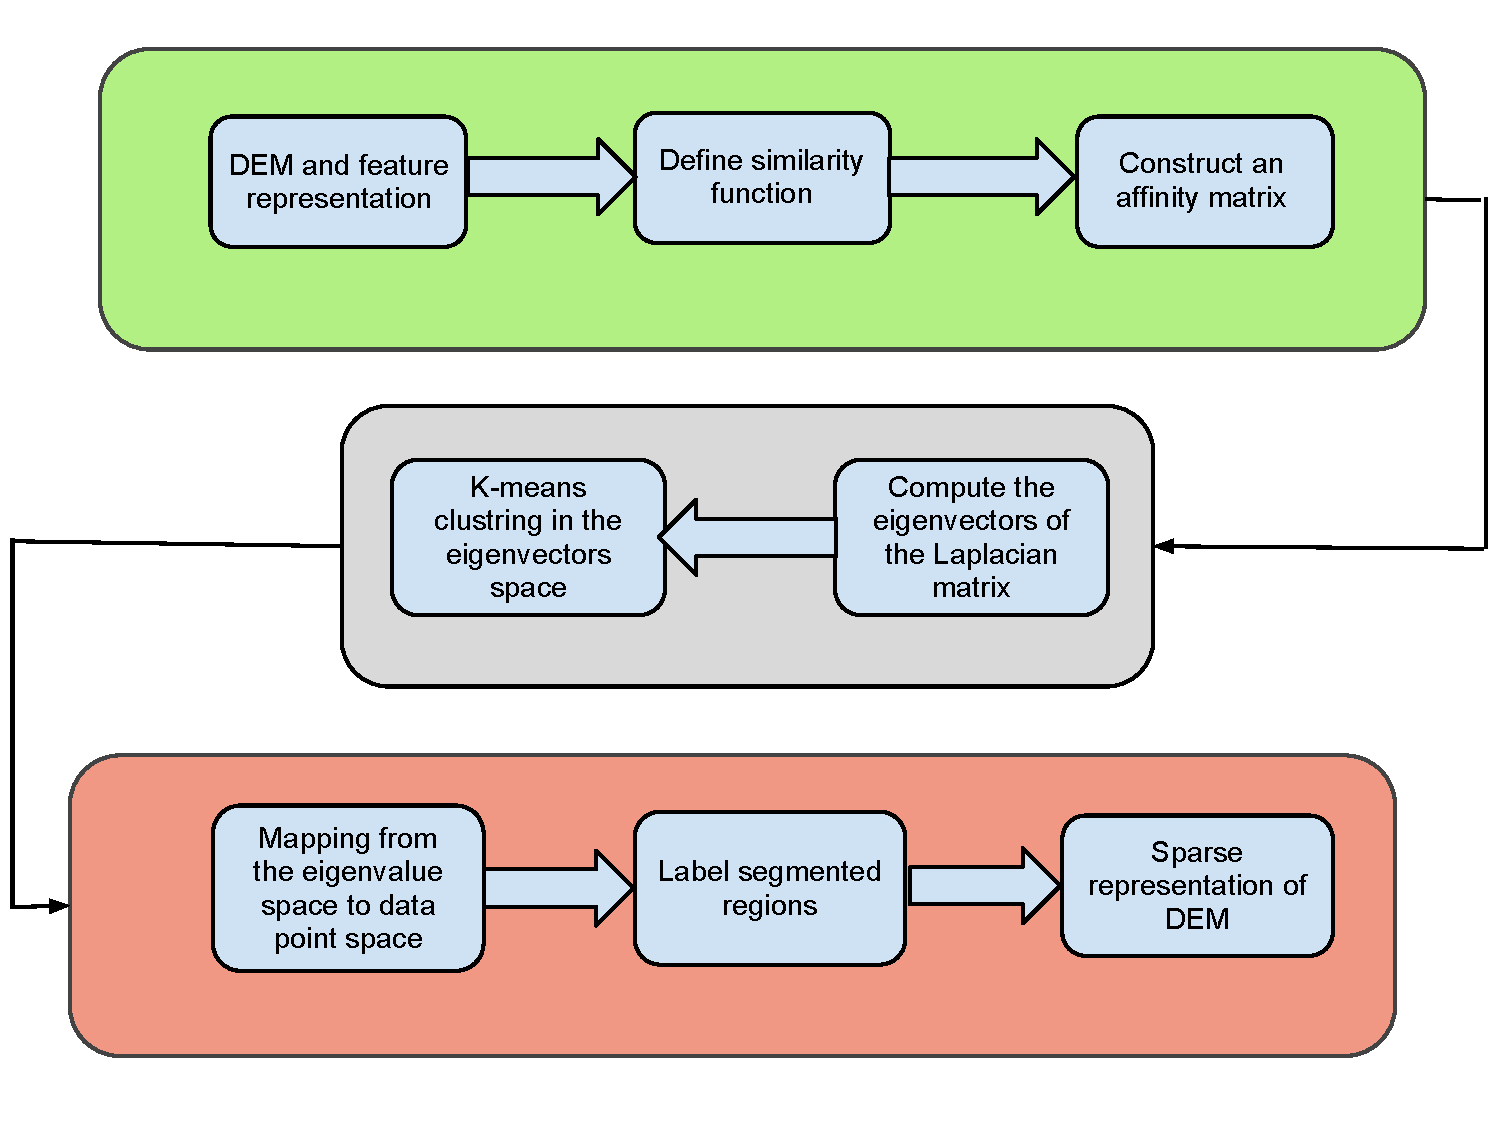
\includegraphics[width=10cm,height=11cm,keepaspectratio]{figs/fig3_pdf.pdf}\\
  \caption{Spectral Clustering workflow}\label{fig:fig2}
\end{figure}
The most interesting aspect of Spectral Clustering is the mapping of the data points into a new space with
$k$-dimensions by means of eigenvector decomposition. 
These eigenvectors induce an embedding of the data points in a low-dimensional subspace wherein a
partitioning based on the Normalized Cut (NCut) can be used. If we let $A$ and $B$ represent a bipartition
of $V$, ($ A \cup B = V$ and $A\cap B = \emptyset$). It can be defined $cut (A, B) =  \sum_{i\in A,j\in B}W_{ij}$ and 
$assoc(A, V) = \sum_{i \in A, j \in V}W_{ij}$. The normalized cut between sets $A$ and $B$ is then given by:
\begin{align}
NCut(A, B) = \frac{cut(A, B)}{assoc(A, V)} + \frac{cut(A, B)}{assoc(B, V)}
\end{align}
The problem is to find $A$ and $B$ such that $NCut(A, B)$ is minimized. The solution of this problem can be 
obtained from the Fiedler eigenvector [9].
 
%In Figure~\ref{fig:fig3} the Spectral Clustering was performed for $\sigma=1$ and a DEM of 120m resolution. 
%\begin{figure}[ht!]
%\center
%      \includegraphics[width=10cm,height=11cm,keepaspectratio]{Spectral1.pdf}\\
%  \caption{Spectral Clustering $\sigma =1 $  }\label{fig:fig3}
%\end{figure}
%\begin{figure}[ht!]
%  \begin{minipage}[b]{0.5\textwidth}
%    \begin{tabular}{c}
%      \includegraphics[width=7cm,height=8cm,keepaspectratio]{pics/T5_K4.pdf}\\
%      (a)
%    \end{tabular}
%  \end{minipage}
%  % \hfill
%  \begin{minipage}{0.5\textwidth}
%    \begin{tabular}{c}
%      \includegraphics[width=7cm,height=8cm,keepaspectratio]{pics/T5_K6.pdf}\\
%      (b)
%    \end{tabular}
%  \end{minipage}
%  \caption{a) Hillshade plot of the Mammoth Mountain b) 3D plot Mammoth Mountain }\label{fig:fig1}
%end{figure}
%As a next step in our project we will try to improve the way the affinity matrix is define in spectral clustering,
%such that both location and the feature matrix to be incorporated. Also, a Gaussian Mixture clustering will be
%implemented.

\section{Results and Conclusions}

The data set available is a 5m DEM, covering an area of $\approx 94 km^2$ which results in $\approx 3$ millions 
data points. To speed up the computational time, the majority of the analysis was performed on a decimated 
DEM having a 120m resolution and 6550 data points. 

The implementation of equation 11 it is still a work in progress. 
We succeeded in performing the classic EM Gaussian Mixture (EMGM) on the \textit{feature matrix} 
$X = \{x_k | 1\le k \le N\}$ with dimensionality $d$,
where $x_k$ is a $d \times 1$ matrix. In this case $d=4$ and $N=6550$. 
The feature were previously scaled such that their means were equal to zero.
The initial parameters were chosen from the results of $K$-means results. The results are presented in Figure~\ref{fig:fig3} (b) and are compared to the Matlab build-in function 
(Fig. ~\ref{fig:fig3} (a)).
The results are quite different and we assume that using $K$-means for parameter initialization makes a significant difference in the clustering process.
Also, adding more geomorphometric features results in differing assignments of data points to clusters.

\begin{figure}[ht!]
  \begin{minipage}[b]{0.5\textwidth}
    \begin{tabular}{c}
      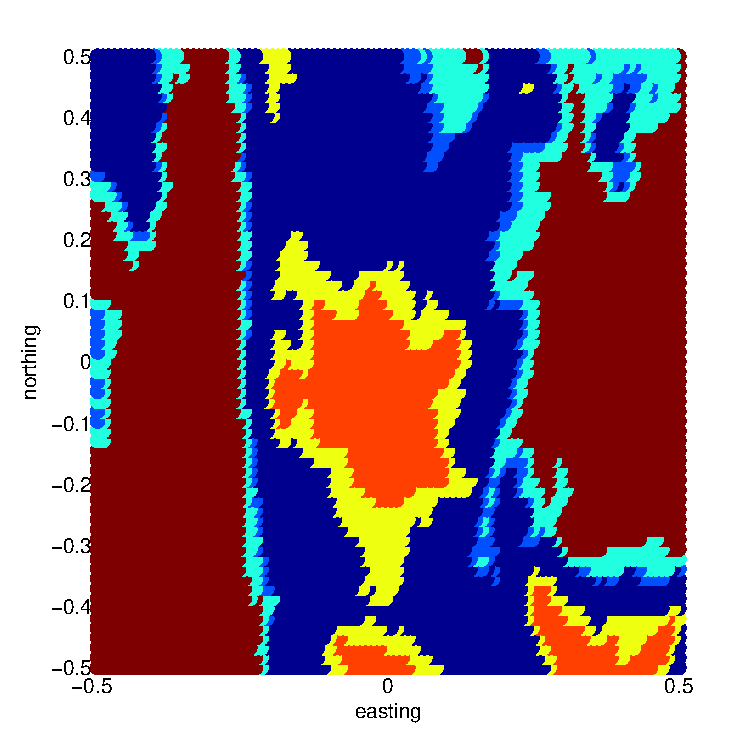
\includegraphics[width=8cm,height=7cm,keepaspectratio]{figs/GM_matlab.pdf}\\
      (a)
    \end{tabular}
  \end{minipage}
  % \hfill
  \begin{minipage}{0.5\textwidth}
    \begin{tabular}{c}
      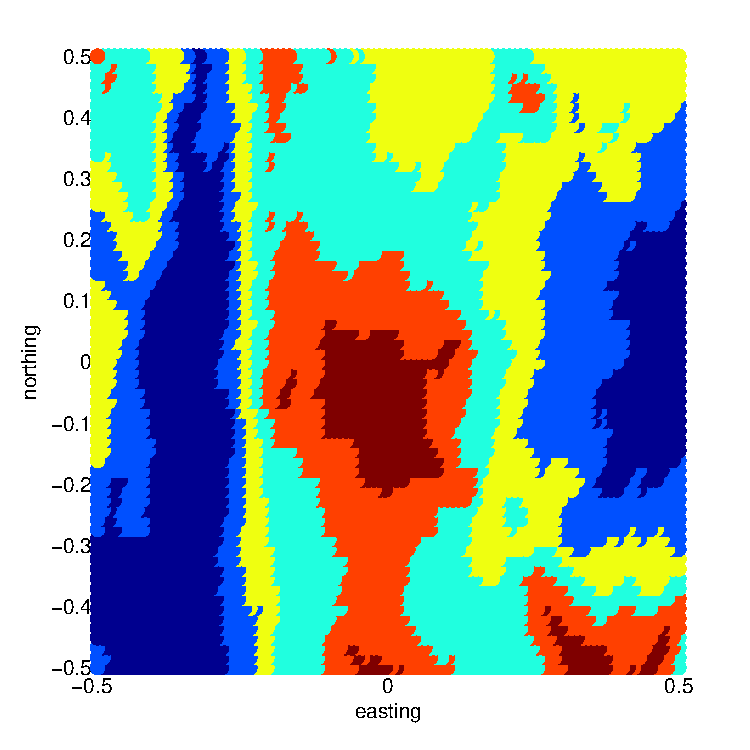
\includegraphics[width=8cm,height=7cm,keepaspectratio]{figs/GM_me.pdf}\\
      (b)
    \end{tabular}
  \end{minipage}
  \begin{minipage}[b]{0.5\textwidth}
    \begin{tabular}{c}
      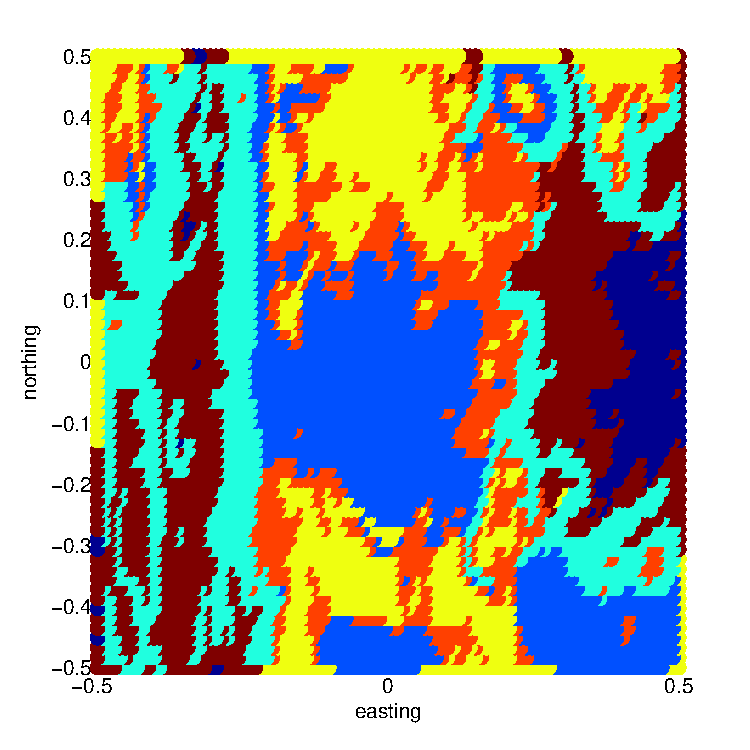
\includegraphics[width=8cm,height=7cm,keepaspectratio]{figs/GM_me_feat_2.pdf}\\
      (c)
    \end{tabular}
  \end{minipage}
  % \hfill
  \begin{minipage}{0.5\textwidth}
    \begin{tabular}{c}
      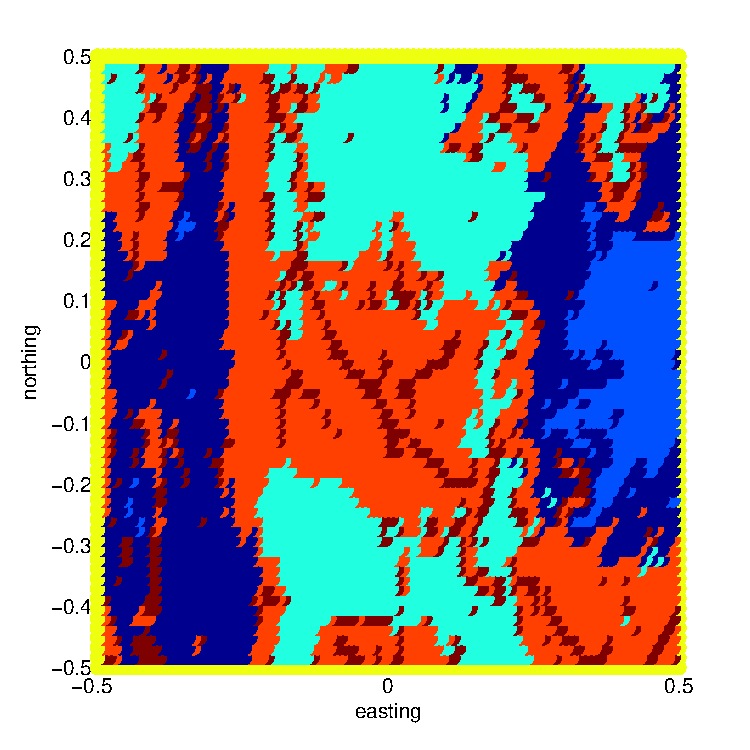
\includegraphics[width=8cm,height=7cm,keepaspectratio]{figs/GM_me_feat_4.pdf}\\
      (d)
    \end{tabular}
  \end{minipage}
   \caption{EM Gaussian Model clustering for a) K=6 using Matlab build in function for one feature (elevation) \textit{gmdistribution} b) K=6 using an improved EMGM -- one feature (elevation)  c) K=6 using 2 features (elevation and slope)  d) K=6 using 4 feature (elevation, slope, transversal, and profile curvature) }\label{fig:fig3}
\end{figure}

Spectral Clustering was performed for $K=6$ and $K=20$ (Fig. ~\ref{fig:fig4} (a), (b)). We observe that classical EMGM clustering (Fig.~\ref{fig:fig3} (b)) and Spectral Clustering (Fig.~\ref{fig:fig4} (a)) give similar results which give us confidence of the \textit{goodness of fit} for those methods, considering that we had not used any performance measures. 
Spectral Clustering requires setting a set of parameters, namely, the scaling parameters $\sigma_F$ and $\sigma_x$. These parameters are very important since they add more weigh to the features that we consider that are more important than the others.
Appropriate setting of $\sigma$ is crucial for obtaining good segmentation results in Spectral Clustering. Unfortunately, it is
difficult to choose the appropriate $\sigma$ value, and it is always set manually. The incorrect value of  $\sigma$ can degrade the performance as the Spectral Clustering is highly sensitive to $\sigma$, and different values of 
$\sigma$ may lead to drastically different results (Fig. ~\ref{fig:fig4} (c), (d)). The proper setting of the scaling parameter still remains an open issue, and there is no known effective method.
 
\begin{figure}[ht!]
  \begin{minipage}[b]{0.5\textwidth}
    \begin{tabular}{c}
      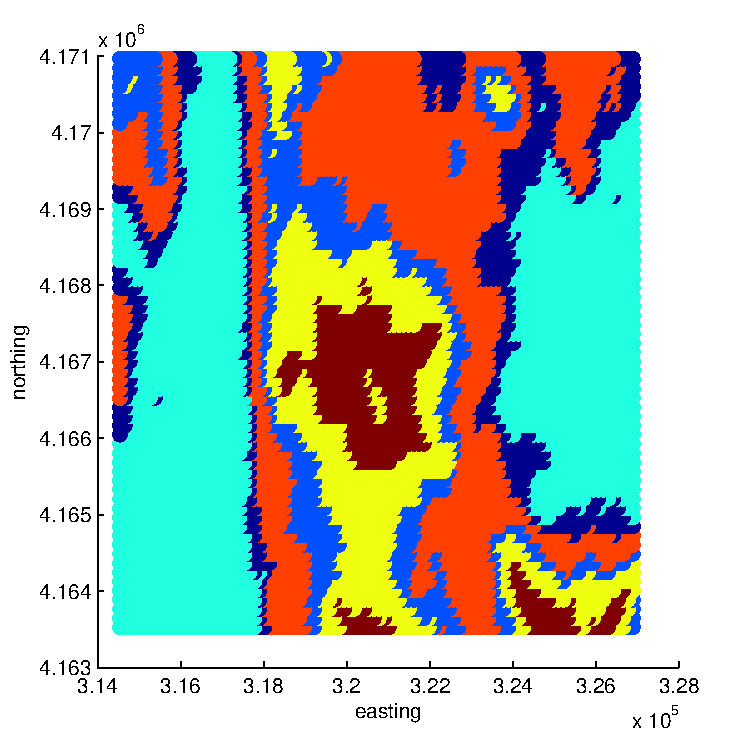
\includegraphics[width=8cm,height=7cm,keepaspectratio]{figs/Spectral1_old.pdf}\\
      (a)
    \end{tabular}
  \end{minipage}
  % \hfill
  \begin{minipage}{0.5\textwidth}
    \begin{tabular}{c}
      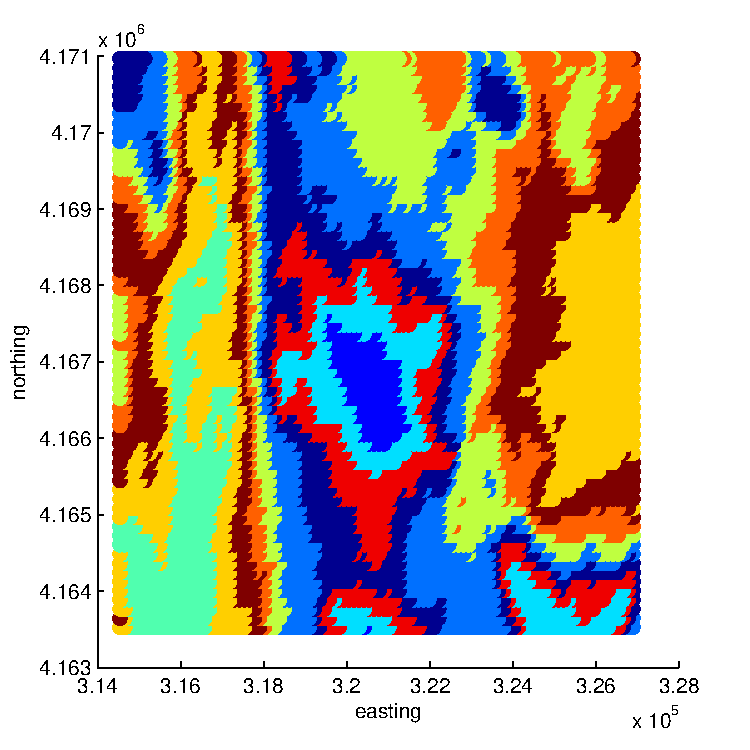
\includegraphics[width=8cm,height=7cm,keepaspectratio]{figs/T30_K10.pdf}\\
      (b)
    \end{tabular}
  \end{minipage}
  \begin{minipage}[b]{0.5\textwidth}
    \begin{tabular}{c}
      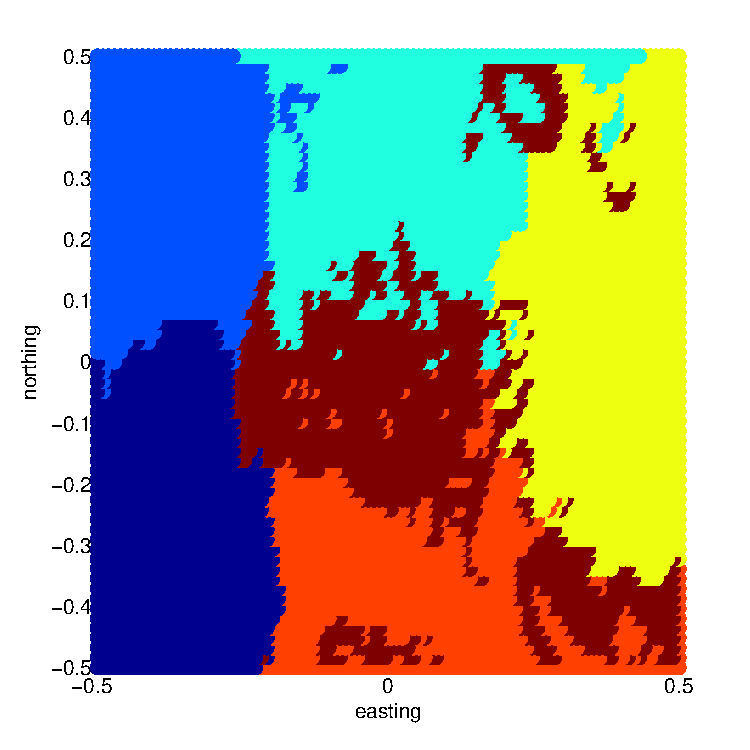
\includegraphics[width=8cm,height=7cm,keepaspectratio]{figs/Spectral2.pdf}\\
      (c)
    \end{tabular}
  \end{minipage}
  % \hfill
  \begin{minipage}{0.5\textwidth}
    \begin{tabular}{c}
      \includegraphics[width=8cm,height=7cm,keepaspectratio]{figs/Spectral1.pdf}\\
      (d)
    \end{tabular}
  \end{minipage}
   \caption{Spectral Clustering for a) K=6 -- one feature b) K=20 -- one feature c) K=6  where $\sigma_F = 0.8$ and $\sigma_x = 1$ -- 4 feature d) K=6  $\sigma_F = 0.8$ and $\sigma_x = 0.8$ -- 4 feature}\label{fig:fig4}
\end{figure}

\section*{Acknowledgment}
 

\subsubsection*{References}
\small{
%[1] Ambroise, C., Dang, M. \& Govaert, G. (1996) Clustering of spatial
%data by the EM algorithm. {\it Geostatistics for Environmental Applications},
%pp. 493-504.

[1] Junior, E.R.S., Cavalcanti, G.D.C. \& Ren, T.I. (2010) Does the affinity matrix
influence the performance of the Locality Preserving Projection algorithm? 
{\it IEEE International Conference on Systems, Man, and Cybernetics (SMC)}, Istanbul. 

[2] von Luxburg, U. (2007) A Tutorial on Spectral Clustering. {\it Statistics 
and Computing} {\bf 17}.

[3] MacQueen, J.B. Some methods for classification and analysis of multivariate 
observations. {\it in Berkley Symposium on Mathematical Statistics and Probability},
vol.1.

[4] Ng, A.Y., Jordan, M.I., \& Weiss, Y. (2002) On Spectral Clustering: Analysis
and an algorithm. {\it NISP} {\bf14}.

[5] Archip, N., Rohling R., Cooperberg P., Tahmasebpour H., Warfield S.K. (2005) Spectral 
Clustering Algorithms for Ultrasound Image Segmentation. 
{\it Int Conf Med Image Comput Comput Assist Interv.} {\bf 8(Pt 2)}:862-9. PMID: 16686041

[6]  Bishop, C. M.,(2007) Pattern Recognition and Machine Learning, {\it Springer}

[7] Sujaritha, M., S., Annadurai (201) Color Image Segmentation using Adaptive Spatial
Gaussian Mixture Model, {\it Int Journal of Information and Comm Eng.} {\bf 6:1}

[8] Tung, F., A. Wong \& D. A., Clausi (2010) Enabling scalable spectral clustering for image
 segmentation {\it Pattern Recognition} {\bf 43}, 4069-4076

[9] Xiangrong, Z., L., Jiao, L., Bo \& M., Gong Spectral clustering ensemble applied to SAR
 image segmentation.% {\it MS (w) GBIS (x) Consensus}
}



%\bibliographystyle{plainnat} \bibliography{myrefs}
\end{document}